\chapter{Experimental Results} \label{chap:results}

\section{Experiment setup}
\subsection{Datasets}

%we utilized as shown in the table, remove the other part
In order to validate the experimental methods discussed in this thesis, we utlized various datasets as shown in Table \ref{table:expData}. 


\begin{table}[ht]
\caption{Summary of experimental datasets} % title of Table
\centering % used for centering table
\begin{tabular}{l l l l l l} % centered columns (4 columns)
\hline %inserts single horizontal lines
Experiment & Bimodal dataset & Method & Samples & Classes & Feature type \\ %[0.5ex] % inserts table
%heading
\hline % inserts single horizontal line
\hyperlink{subsec:classA}{Sec. \ref{subsec:classA}} & CNV + miRNA-seq & DCF & 3988 & 9 & real\\ 
\hyperlink{subsec:classA}{Sec. \ref{subsec:classA}} & CNV + miRNA-seq & SDAE & 3988 & 9 & real\\ 
\hyperlink{subsec:gmuComp}{Sec. \ref{subsec:gmuComp}} & RNA-seq + miRNA-seq & DE & 3988 & 9 & real\\ 
\hyperlink{subsec:dgmuInt}{Sec. \ref{subsec:dgmuInt}} & RNA-seq + SNV & DE + CGF & 3375 & 6 & real + integer\\ 
%Exp7 & dp & fet & - & regression     & real\\ 
[1ex]   % [1ex] adds vertical space 
\hline %inserts single line
\end{tabular}
\label{table:expData}
\end{table}

\subsection{Metrics}

In these experiments, all models performed multinomial classification. In order to use binary performance metrics, a one-vs-all approach was taken with the model predictions. This approach involves treating each individual prediction as a binary classification where samples of the correct class are positive and all other samples are negative. This strategy works because for each input example the models output a $k$-dimensional vector of real-valued confidence scores for each of the $k$ classes. The predicted output is then designated as the label $k$ for which the classifier reports the largest confidence score:

\begin{equation*}
    \hat{y} =  \underset{k \in \{ 1 \dotsc K \}}{\mathrm{argmax}}f_k(x) 
\end{equation*}

\noindent
This strategy creates a particular problem related to class distribution in the training set. Treating each classification as a binary prediction results in an unbalanced distribution. The set of negatives examples will be much larger than the set of positive examples \cite{bishop2006pattern}. As well, the distribution of labels between the cell types are not equal. This can lead to issues when evaluating models if the accuracy is the only measure of performance. In order to avoid issues related to class imbalance, the precision, recall, and $F_1$ score were also used as performance metrics. The $F_1$ score is the harmonic mean of the recall and precision:

\begin{equation*}
F_1 = \left ( \frac{recall^{-1} + precision^{-1}}{2} \right )^{-1}
\end{equation*},

\noindent
where the precision and recall are defined as:

\begin{equation*}
    precision = \frac{true \; positives}{true \; positives + false \; positives} \;\;\;\;\; recall = \frac{true \; positives}{true \; positives + false \; negatives}
\end{equation*}

\noindent
Furthermore, in order to visualize the performance of the multinomial cell type classifications we used area under the curve (AUC) receiver operating characteristics (ROC). AUC-ROC plots provide a performance measurement at various statistical thresholds. These measurements indicates how much the model is capable of discerning between classes. The higher the AUC, the better the model is at classifying true positives as positive and true negatives as negative. ROC curves are produced by plotting the true positive rate (TPR) on the y-axis, and the false positive rate (FPR) on the x-axis. The TPR is equivalent to $recall$, and the FPR is equal to $1 - specificity$:

\begin{equation*}
    specificty = \frac{true \; negatives}{true \; negatives + false positives} \;\;\;\;\; FPR = \frac{false \; positives}{true \; negatives + false \; positives}
\end{equation*}

\noindent
A perfect model has an AUC of 1. This means that the model can perfectly separate $true negatives$ and $true positives$ samples 100\% of the time. This results in a ROC curve where $TPR = 1$ for $FPR \in {0,1}$. The closer the top left corner of the ROC plot is to the point (0,1), the better the model. An AUC of 0.5 means the model does not have the capacity to separate the classes. In this case, the model predictions are essentially assigned by random chance. On the ROC plot, an AUC of 0.5 results in a straight diagonal line.

In order to extend the ROC for multi-class classification, a pairwise comparison was performed to binarize the output of the classification. Here a one versus all approach was taken to compute the ROC for individual cancer cell tissue types \cite{allwein2000reducing}. Accordingly, the models were evaluated for their ability to classify an individual cell tissue type against all other cell tissue types. ROC curves were also drawn using micro-averaging, where each element of the model classification was considered as a binary prediction, and macro-averaging, which finds the unweighted mean of all class ROCs.

\section{Results}

In the following, we report the results from all experiments. In all cases, experiments were constructed using the following experimental settings and constraints:

\begin{itemize}
    \item The datasets were divided into a 60/20/20 split for training, validation, and testing, respectively.
    \item Hyperparameter tuning was performed on the cross validation set.
    \item Experiments were repeated 10 times using 10 fold cross validation on the training set.
\end{itemize}

\subsection{Classification Agreement and Model Performance}\label{subsec:classA}

%%%%%%%%%%%%%%%%%%%%%%%%%%%%%%%%%%%%%%%%%%%%%%%%%%%%%%%%%%%%%%%%%%%%%%%%%%%%
\subsubsection{Comparison of Classification Agreement} 
%%%%%%%%%%%%%%%%%%%%%%%%%%%%%%%%%%%%%%%%%%%%%%%%%%%%%%%%%%%%%%%%%%%%%%%%%%%%

In order to evaluate the effectiveness of the dGMU model, we compared single modality, and bimodality classification agreements for SDAE and DCF reduced miRNA-seq and CNV features. The results for each feature type along with their respective models are summarized on Table \ref{tab:classAgree}. The DCF features were observed to result in higher classification scores for most feature and model type combinations. The only exception was the single modality CNV with SDAE features, which had a higher accuracy, recall, and macro f1-score for MLP and SVM models. Independent of the evaluated feature types, the dGMU model achieved the highest classification metrics amongst the utilized methods.

\begin{table}[h!]
   \caption{Summary of classification agreement for CNV and miRNA-seq reduced to 500 features.} 
   \label{tab:classAgree}
   %\small % text size of table content
   \centering % center the table
   \scalebox{0.9}{
\begin{tabular}{|c|c|c| c c c c |c|}
        \hline
        \multicolumn{3}{|c|}{Experiment}  & \multicolumn{4}{c|}{Classification Metric}\\
        \cline{1-7}
        Modality & Feature & Model & Accuracy & Precision & Recall & F1-Score\\
        \hline
        \multirow{10}{*}{Bimodal} & \multirow{5}{*}{SDAE} & dGMU & 0.8764 &	0.8739 & 0.8749 & 0.8737  \\
                            &                             & GMU  & 0.8722 &	0.8700 & 0.8661 & 0.8675 \\
                            &                             & MoE  & 0.7611 &	0.7617 & 0.7566 & 0.7556  \\
                            &                             & MLP  & 0.8622 &	0.8613 & 0.8542 & 0.8570  \\
                            &                             & SVM  & 0.8605 &	0.8567 & 0.8542 & 0.8550  \\
                                   \cline{2-7}
                                 & \multirow{5}{*}{DCF}   & dGMU & \textbf{0.9373} & \textbf{0.9357} & \textbf{0.9327} & \textbf{0.9341}  \\
                            &                             & GMU  & 0.9273 &	0.9292 & 0.9228 & 0.9255  \\
                            &                             & MoE  & 0.9156 &	0.9109 & 0.9111 & 0.9109  \\
                            &                             & MLP  & 0.9189 &	0.9199 & 0.9123 & 0.9154  \\
                            &                             & SVM  & 0.9172 &	0.9175 & 0.9150 & 0.9136  \\
        \hline
        \multirow{4}{*}{CNV} & \multirow{2}{*}{SDAE}      & MLP & 0.7586 &	0.7622 & 0.7534 & 0.7526   \\
                            &                             & SVM & 0.7343 &	0.7459 & 0.7275 & 0.7321  \\
                                   \cline{2-7}
                                 & \multirow{2}{*}{DCF}   & MLP & 0.7468 &	0.7795 & 0.7270 & 0.7200   \\
                            &                             & SVM & 0.7335 &	0.7460 & 0.7256 & 0.7310  \\
        \hline
        \multirow{4}{*}{miRNA-seq} & \multirow{2}{*}{SDAE}  & MLP & 0.8530 &	0.8560 & 0.8425 & 0.8477   \\
                            &                             & SVM & 0.8429 &	0.8388 & 0.8347 & 0.8362  \\
                                   \cline{2-7}
                                 & \multirow{2}{*}{DCF}   & MLP & 0.9097 & 0.9118 & 0.9022 & 0.9052   \\
                            &                             & SVM & 0.9072 &	0.9104 & 0.9045 & 0.9004  \\
        \hline
    \end{tabular}}
\end{table}

%%%%%%%%%%%%%%%%%%%%%%%%%%%%%%%%%%%%%%%%%%%%%%%%%%%%%%%%%%%%%%%%%%%%%%%%%%%%
\subsubsection{Comparison of Model Performance} 
%%%%%%%%%%%%%%%%%%%%%%%%%%%%%%%%%%%%%%%%%%%%%%%%%%%%%%%%%%%%%%%%%%%%%%%%%%%%

A more exhaustive characterization of the classification performance was achieved with the multi-class receiver operator characteristic (ROC) curves shown in Fig. \ref{fig:c_r_dcf_roc}. The false positive rate versus the true positive rate was plotted for a subset of the best performing models trained with bimodal DCFs reduced to a dimensionality of 500 from miRNA-seq and CNV data sources. In all models, as the true positive rate increased, the false positive rate increased exponentially. In order to compare model performance, it was ideal to observe the rate in which the true positive rate approaches one as the false positive rate increases. The ROC curves for each model shows the trade-off between sensitivity (true positive rate) and the specificity (1 - false positive rate) for each model. Model types that have curves closer to the top left corner indicated a better performance. In Fig. \ref{fig:dcf_dgmu} and \ref{fig:dcf_gmu}, we see that the dGMU and GMU ROC curves cluster more tightly into the top left corner of their plots as opposed to the MLP and MoE ROC plots. In Fig. \ref{fig:dcf_mlp} and \ref{fig:dcf_moe}, the MLP and MoE plots showed a decrease in model performance as the cluster of curves have decreased slopes. This is especially evident by observing the significantly lowered benign ROC curves in the MLP and MoE plots. In this study, it was imperative to maximize the true positive rate while keeping the false positive rate to a minimum. Accordingly, the area under the curve (AUC) was computed for each cell tissue type. The models that utilized GMUs were specifically more effective at classifying benign cell tissue types. The MLP and MoE models struggled with this classification problem resulting in a benign AUC of 0.90 and 0.87, respectively. The GMU based models rectified this deficiency, both resulting in a benign AUC of 0.98. Furthermore, utilizing the ROC averages as a holistic measure of model classification performance, the dGMU model was observed to have the largest macro-average AUC of 0.98 and shared an identical micro-average AUC of 0.98 with the single GMU model. This indicates that the deeper configuration of the GMU improves cell tissue differentiation.

\begin{figure}[h!]
        \centering
         \sidesubfloat[]{\includegraphics[height=5cm,width=0.45\textwidth]{img/c_r/c_r_dcf_dgmu_roc.png}\label{fig:dcf_dgmu}}
        \hfill
         \sidesubfloat[]{\includegraphics[height=5cm,width=0.45\textwidth]{img/c_r/c_r_dcf_gmu_roc.png}\label{fig:dcf_gmu}}
         
        \sidesubfloat[]{\includegraphics[height=5cm,width=0.45\textwidth]{img/c_r/c_r_dcf_mlp_roc.png}\label{fig:dcf_mlp}}
        \hfill
         \sidesubfloat[]{\includegraphics[height=5cm,width=0.45\textwidth]{img/c_r/c_r_dcf_moe_roc.png}\label{fig:dcf_moe}}
         
        \caption{CNV and miRNA-seq DCF bimodal model ROC plots for (a) dGMU (b) GMU (c) MLP and (d) MoE models.}
        \label{fig:c_r_dcf_roc}
\end{figure}

In order to evaluate the impact of feature dimensionality on the performance of the bimodal models, classification experiments were conducted with input dimensionalities ranging from 10 to 1500 features per modality. Fig. \ref{fig:exp82} shows the error rates observed for miRNA-seq and CNV DCF inputs at varying sizes. In all models, as the feature dimensionality increased, the error rate decreased. Though, the error rate stops improving rapidly after an input dimensionality of approximately 500. The dGMU model obtained the lowest error rate at 5.93\%. The dGMU model also demonstrates the highest resistance to decreasing dimensionality, except for in feature sizes ranging from 100 to 200, where the GMU model obtained lower error rates.

\begin{figure}[h!]
    \centering
    \includegraphics[height=5.5cm,width=0.80\textwidth]{img/c_r/exp82.eps}
    \caption{CNV and miRNA-seq DCF model error rates over a range of input dimensionalities.}
    \label{fig:exp82}
\end{figure}

%%%%%%%%%%%%%%%%%%%%%%%%%%%%%%%%%%%%%%%%%%%%%%%%%%%%%%%%%%%%%%%%%%%%%%%%%%%%
\subsubsection{Visualization of dGMU Latent Space} 
%%%%%%%%%%%%%%%%%%%%%%%%%%%%%%%%%%%%%%%%%%%%%%%%%%%%%%%%%%%%%%%%%%%%%%%%%%%%

The latent space produced by the dGMU model was visualized with t-distributed stochastic neighbor embedding (t-SNE) \cite{maaten2008visualizing}. In Fig. \ref{fig:c_r_dcf_tsne}, the dGMU model was shown to have a highly discriminatory latent space. The cell tissue types were largely clustered into the original nine classifications with a perceived level of geometric preservation between related cancers. These relationships include the kidney renal carcinoma's KIRC and KIRP, and the adenocarcinoma's LUAD and PRAD.

\begin{figure}[h!]
        \centering
        %\sidesubfloat[]{\includegraphics[height=6cm,width=0.9\textwidth]{img/c_r/latentHeat.eps}\label{fig:latentHeat}}
        
         \sidesubfloat[]{\includegraphics[width=0.45\textwidth]{img/c_r/c_r_dcf_tsne.png}\label{fig:c_r_dcf_tsne}}
        \hfill
         \sidesubfloat[]{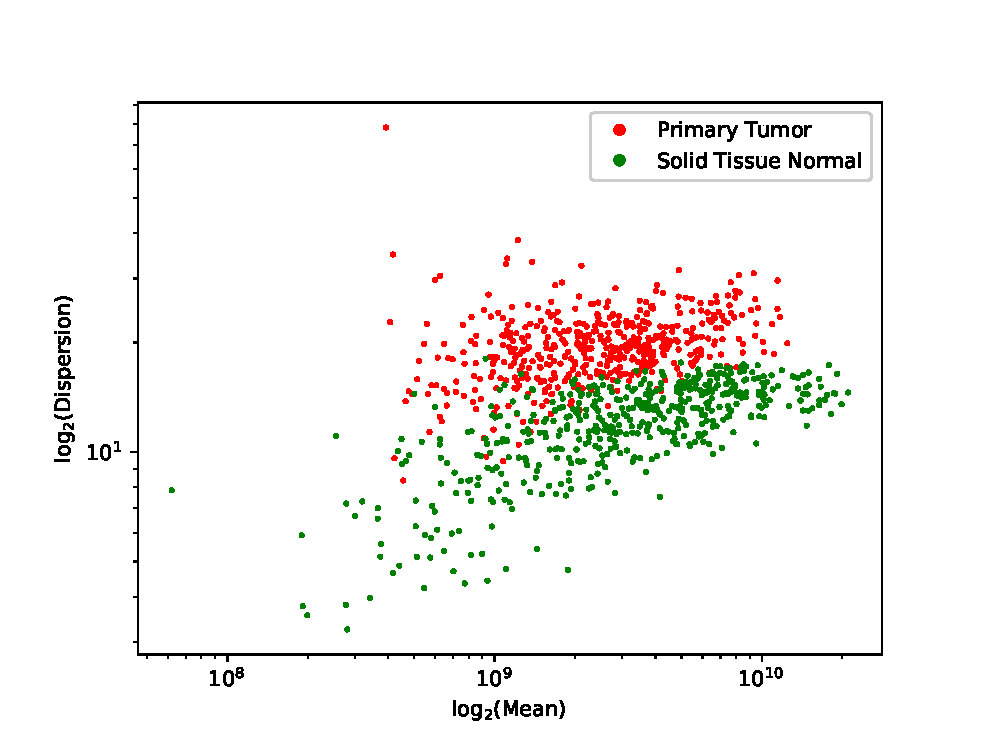
\includegraphics[width=0.45\textwidth]{img/c_r/c_r_disp.eps}\label{fig:c_r_dcf_disp}}
         
        \caption{(a) CNV and miRNA-seq DCF dGMU model latent space clustered with t-distributed stochastic neighbor embedding (t-SNE). (b) Fold change and dispersion of the dGMU latent space.}
        \label{fig:visLate}
\end{figure}

%reference the color in the text

In order to evaluate inherit characteristics of the latent space, we considered the dispersion and the mean of the fusion encodings. In Fig. \ref{fig:c_r_dcf_disp}, the dispersion was plotted against the log mean encoded value. The dissemination of the latent encoding was stratified in relation to the log$_2$(Dispersion) and the log$_2$(Mean). Distinct clusters were observed with labeled red and green markers for the samples derived from primary tumours and normal tissue, respectively. The dispersion values scatter with a degree of variance, which was expected given the sample size between the primary tumour and solid tissue normal samples \cite{jiang2014statistical}.

%%%%%%%%%%%%%%%%%%%%%%%%%%%%%%%%%%%%%%%%%%%%%%%%%%%%%%%%%%%%%%%%%%%%%%%%%%%%
\subsection{GMU Model Comparison}\label{subsec:gmuComp}
%%%%%%%%%%%%%%%%%%%%%%%%%%%%%%%%%%%%%%%%%%%%%%%%%%%%%%%%%%%%%%%%%%%%%%%%%%%%

%%%%%%%%%%%%%%%%%%%%%%%%%%%%%%%%%%%%%%%%%%%%%%%%%%%%%%%%%%%%%%%%%%%%%%%%%%%%
\subsection{dGMU Model Interpretation}\label{subsec:dgmuInt}
%%%%%%%%%%%%%%%%%%%%%%%%%%%%%%%%%%%%%%%%%%%%%%%%%%%%%%%%%%%%%%%%%%%%%%%%%%%%

Methods
The predictive behaviour of the dGMU model is examined using a linear model to approximate the decision boundary in the neighborhood of each correctly labeled instance.

We examined the functional enrichment of the top 400 interpretable gene components through a GO term and KEGG pathway analysis. The top 400 genes that promote positive explanations for the eight cancer types were identified as having significantly enriched GO terms and related pathways. The biological process related GO terms with a p-value smaller than $10^{-10}$ and the related KEGG pathways with p-value smaller than $10^{-3}$ are presented on Table \ref{tab:goTab}. Many of the statistically significant pathways and terms are related to DNA replication, DNA repair, and cell cycle processes. This suggests that the genes most attributed to explaining the cancer classifications are related to cell proliferation and tumor growth. Furthermore, an additional review of literature was used to identify relationships between the significantly enriched pathways and the cancer types. The enrichmenet analysis for LIHC identified the carbon metabolism (hsa01200) KEGG pathway, and the response to insulin (GO:0032868), response to activity (GO:0014823), and fatty acid metabolic process (GO:0006631) GO terms. The identification of these biological processes support significant research describing the pathophysiological link between the human bodies response to insulin and the incidence of LIHC \cite{li2017diabetes,singh2018diabetes}. Insulin stimulates the liver to store glucose, and the liver is the primary site for converting excess carbohydrates into fatty acids. Dysregulated cellular metabolism, where abberant oncogenic signals alter the expression of metabolic enzymes, is a reoccurring theme in cancer cells. Currently, there is substantial evidence supporting dysregulated fatty acid metabolism and lipid metabolic reprogramming in LIHC \cite{wang2016dysregulated,nakagawa2018lipid}. Through the application of LIME, we identified that the dGMU model is using biologically relevant information to stratify cancer classifications. These results suggest that a domain expert can use the interpretable gene components to understand why the dGMU model correctly classifies true positive cancer instances.\\

\begin{table}[h!]
   \caption{Summary of enriched gene ontology terms and related pathways.} 
   \label{tab:goTab}
   %\small % text size of table content
   \begin{adjustbox}{max width=\textwidth}
   \centering % center the table
\begin{tabular}{|c|c|c| c c c |c|c|}
        \hline
        \multirow{2}{*}{Cancer Name}  & \multicolumn{6}{c|}{Enriched GO term and Related Pathway}\\
         \cline{2-7}
                                      & ID & \multicolumn{3}{c|}{Name} & Enrichment & P-value\\
        \hline
        \multirow{6}{*}{HNSC} & hsa04110 & \multicolumn{3}{c|}{Cell cycle} & 5.2 & 4.1E-5\\
                              & hsa03030 & \multicolumn{3}{c|}{DNA replication} & 9.8 & 3.1E-4\\
                              & hsa04914 & \multicolumn{3}{c|}{Progesterone-mediated oocyte maturation} & 5.4 & 6.2E-4\\
                              & GO:0051301 & \multicolumn{3}{c|}{Cell division} & 4.7 & 3.3E-11\\
                              & GO:0007062 & \multicolumn{3}{c|}{Sister chromatid cohesion} & 9.2 & 8.3E-11\\
                              & GO:0008283 & \multicolumn{3}{c|}{Cell population proliferation} & 4.4 & 4.3E-15\\
        \hline
        \multirow{2}{*}{KIRC} & GO:0007162 & \multicolumn{3}{c|}{Negative regulation of cell adhesion} & 16.5 & 1.8E-13\\
                              & GO:0001666 & \multicolumn{3}{c|}{Response to hypoxia} & 4.4 & 5.3E-13\\
        \hline
        \multirow{4}{*}{KIRP} & hsa04210 & \multicolumn{3}{c|}{Apoptotic process} & 18.2 & 1.3E-5\\
                              & hsa04914 & \multicolumn{3}{c|}{Progesterone-mediated oocyte maturation} & 5.4 & 6.2E-4\\
                              & GO:0051301 & \multicolumn{3}{c|}{Cell division} & 4.7 & 3.3E-11\\
                              & GO:0007062 & \multicolumn{3}{c|}{Sister chromatid cohesion} & 9.2 & 8.3E-11\\
        \hline
        \multirow{4}{*}{LIHC} & hsa01200 & \multicolumn{3}{c|}{Carbon metabolism} & 6.4 & 7.04E-4\\
                              & GO:0032868 & \multicolumn{3}{c|}{Response to insulin} & 8.6 & 2.6E-13\\
                              & GO:0014823 & \multicolumn{3}{c|}{Response to activity} & 10.8 & 5.9E-13\\
                              & GO:0006631 & \multicolumn{3}{c|}{Fatty acid metabolic process} & 8.9 & 1.0E-12\\
        \hline
        \multirow{5}{*}{LUAD} & hsa00630 & \multicolumn{3}{c|}{Glyoxylate and dicarboxylate metabolism} & 11 & 9.7E-4\\
                              & GO:0001525 & \multicolumn{3}{c|}{Angiogenesis} & 4.1 & 1.9E-14\\
                              & GO:0031568 & \multicolumn{3}{c|}{G1/S transition of mitotic cell cycle} & 5.9 & 4.1E-14\\
                              & GO:0007062 & \multicolumn{3}{c|}{Sister chromatid cohesion} & 6.4 & 2.5E-15\\
                              & GO:0051301 & \multicolumn{3}{c|}{Cell division} & 6.0 & 8.2E-15\\
        \hline
        \multirow{4}{*}{LUSC} & hsa03440 & \multicolumn{3}{c|}{Homologous recombination} & 28.2 & 8.6E-6\\
                              & hsa03030 & \multicolumn{3}{c|}{DNA replication} & 13.6 & 1.9E-4\\
                              & GO:0051301 & \multicolumn{3}{c|}{Cell division} & 5.4 & 2.8E-17\\
                              & GO:0000724 & \multicolumn{3}{c|}{Double-strand break repair via homologous recombination} & 16.4 & 2.3E-14\\
        \hline
        \multirow{1}{*}{PRAD} & hsa04530 & \multicolumn{3}{c|}{Tight junction} & 6.5 & 2.2E-4\\
        \hline
        \multirow{3}{*}{THCA} & GO:0006260 & \multicolumn{3}{c|}{DNA replication} & 10.2 & 3.3E-12\\
                              & GO:0006974 & \multicolumn{3}{c|}{Cellular response to DNA damage stimulus} & 4.4 & 5.03E-13\\
                              & GO:0006915& \multicolumn{3}{c|}{Apoptotic process} & 2.5 & 1.1E-12\\
        \hline
    \end{tabular}
    \end{adjustbox}
\end{table}

The cell division (GO:0051301) GO term was found to be significantly enriched in four cancer types. For HNSC, the pathway related genes were BUB1, LIG1, BIM, CIB1, SAC3D1, SPC24, BORA, BIRC, ECT2, KIF14, BUB3, and NCAPG. For KIRP, the genes were MAD2L2, ZWINT, CDCA3, CDK5, CDK7, KIRF2C, PARD3B, PRKCE, CDT1, BUB1, and TACC1. For LUAD, the genes were ATAD3B, BUB1B, BUB1, DSN1, NEK2, BIRC5, CDC25C, CDC6, CHEK2, KIF18B, NCAPG, RCC1, SGO1, UBE2C. Lastly, for LUSC the genes were ATAD3B, BUB1, LIG1, DSN1, MAD2L2, SPC25, ZWINT, MCM5, PRKCE, RCC2, TACC1, UBE2C. The greatest overlapping similarity were shared between the two lung cancers LUAD and LUSC, where four genes were shown to be shared. Despite representing the same biological process related to cell division, between the four cancer types, the gene sets were observed to be quite heterogeneous. This suggests that the genes identified as interpretable components have potential applications as biomarkers.

\begin{figure}[h!]
    \centering
    \includegraphics[width=\textwidth]{img/top3gene2.eps}
    \caption{Top 3 explanatory genes for each cancer class.}
    \label{fig:top3gene}
\end{figure}

The intuition of the dGMU model was further investigated by examining the top three explanatory genes derived from LIME analysis for each cancer class. The weighted contribution of these genes along with their respective $\mathrm{log}_2\mathrm{FC}$ from the differential expression analysis are shown in Fig. \ref{fig:top3gene}. For HNSC, CDC25A was identified as one the explanatory genes. CDC25A is a protein coding gene and the gene product performs an integral role in cell cycle progression. In literature, CDC25A is a known oncogene that is overexpressed in head and neck cancers \cite{gasparotto1997overexpression}. This validates the explanation derived from the model that found CDC25A as a key explanatory gene with an overexpressed $\mathrm{log}_2\mathrm{FC}$ of 5.9. For THCA, LIME identified PRKCQ and BMP1 as the top two explanatory genes for the dGMU model. PRKCQ has been identified as having a potential role in the progression of thyroid cancer, and BMP1 is a known oncogene with potential gene interactions that are influential in the carcinogenisis of thyroid cancer \cite{xu2014identification,firek2017pathologic}. For both KIRC and KIRP the top explanatory genes, TTYH3 and ALDH2, were identified as prognostic markers for kidney cancer \cite{uhlen2017pathology}. Accordingly, through the application of LIME explanations, the dGMU model has shown a substantial utility of biologically relevant information for predicting cancer type class.

\begin{figure}[h!]
    \centering
    \includegraphics[width=\textwidth]{img/embgene2.eps}
    \caption{2D embedding of RNA-seq and explanation heatmap with a localization of persistent explanations.}
    \label{fig:2dheatmap}
\end{figure}

The location and variability of explanations were visualized using 2D embeddings of the RNA-seq input data. The RNA-seq data were embedded into 2D images by ordering the genes based on gene function and then reshaping the 3025 $\times$ 1 arrays into 55 $\times$ 55 images. An example is shown for five correctly classified HNSC RNA-seq profiles in Fig. \ref{fig:2dheatmap}. The first row shows the 2D embedding of the RNA-seq instances and the second row shows the respective top five positive and negative gene explanations. On the second row, the positive gene explanations that encouraged the prediction of the correct class were labeled in red, and the negative gene explanations were labeled in blue. The circled regions indicate a cluster with a high density of explanatory genes between examples. Although the explanatory genes were determined locally for a given instance, a general consistency in positive explanations remained between RNA-seq data input. 

\begin{figure}[h!]
        \centering
        \includegraphics[width=0.8\textwidth]{img/weightdisth6.eps}
         
        \caption{Distribution of cumulative contribution for positive explanations over a range of training epochs.}
        \label{fig:weightdist_error}
\end{figure}

During the dGMU model training scheme, the cumulative weighted contributions for the RNA-seq and SNV features were examined. We found that as the model increased in efficacy, the influence of the RNA-seq modality increasingly dominated in weighted contribution as shown in Fig. \ref{fig:weightdist_error}. The red kernel density function for the RNA-seq modality progressively separates and settles at a larger average value than the blue kernel density function for the SNV modality. This suggests that the RNA-seq modality contributes stronger explanatory information on average than the SNV modality. This makes sense as the baseline linear model obtained a higher accuracy with the RNA-seq modality than the SNV modality as shown by the associated line chart of error rates illustrated alongside the labelled training epochs on Fig. \ref{fig:weightdist_error}. 
\begin{figure}[h!]
    \centering
    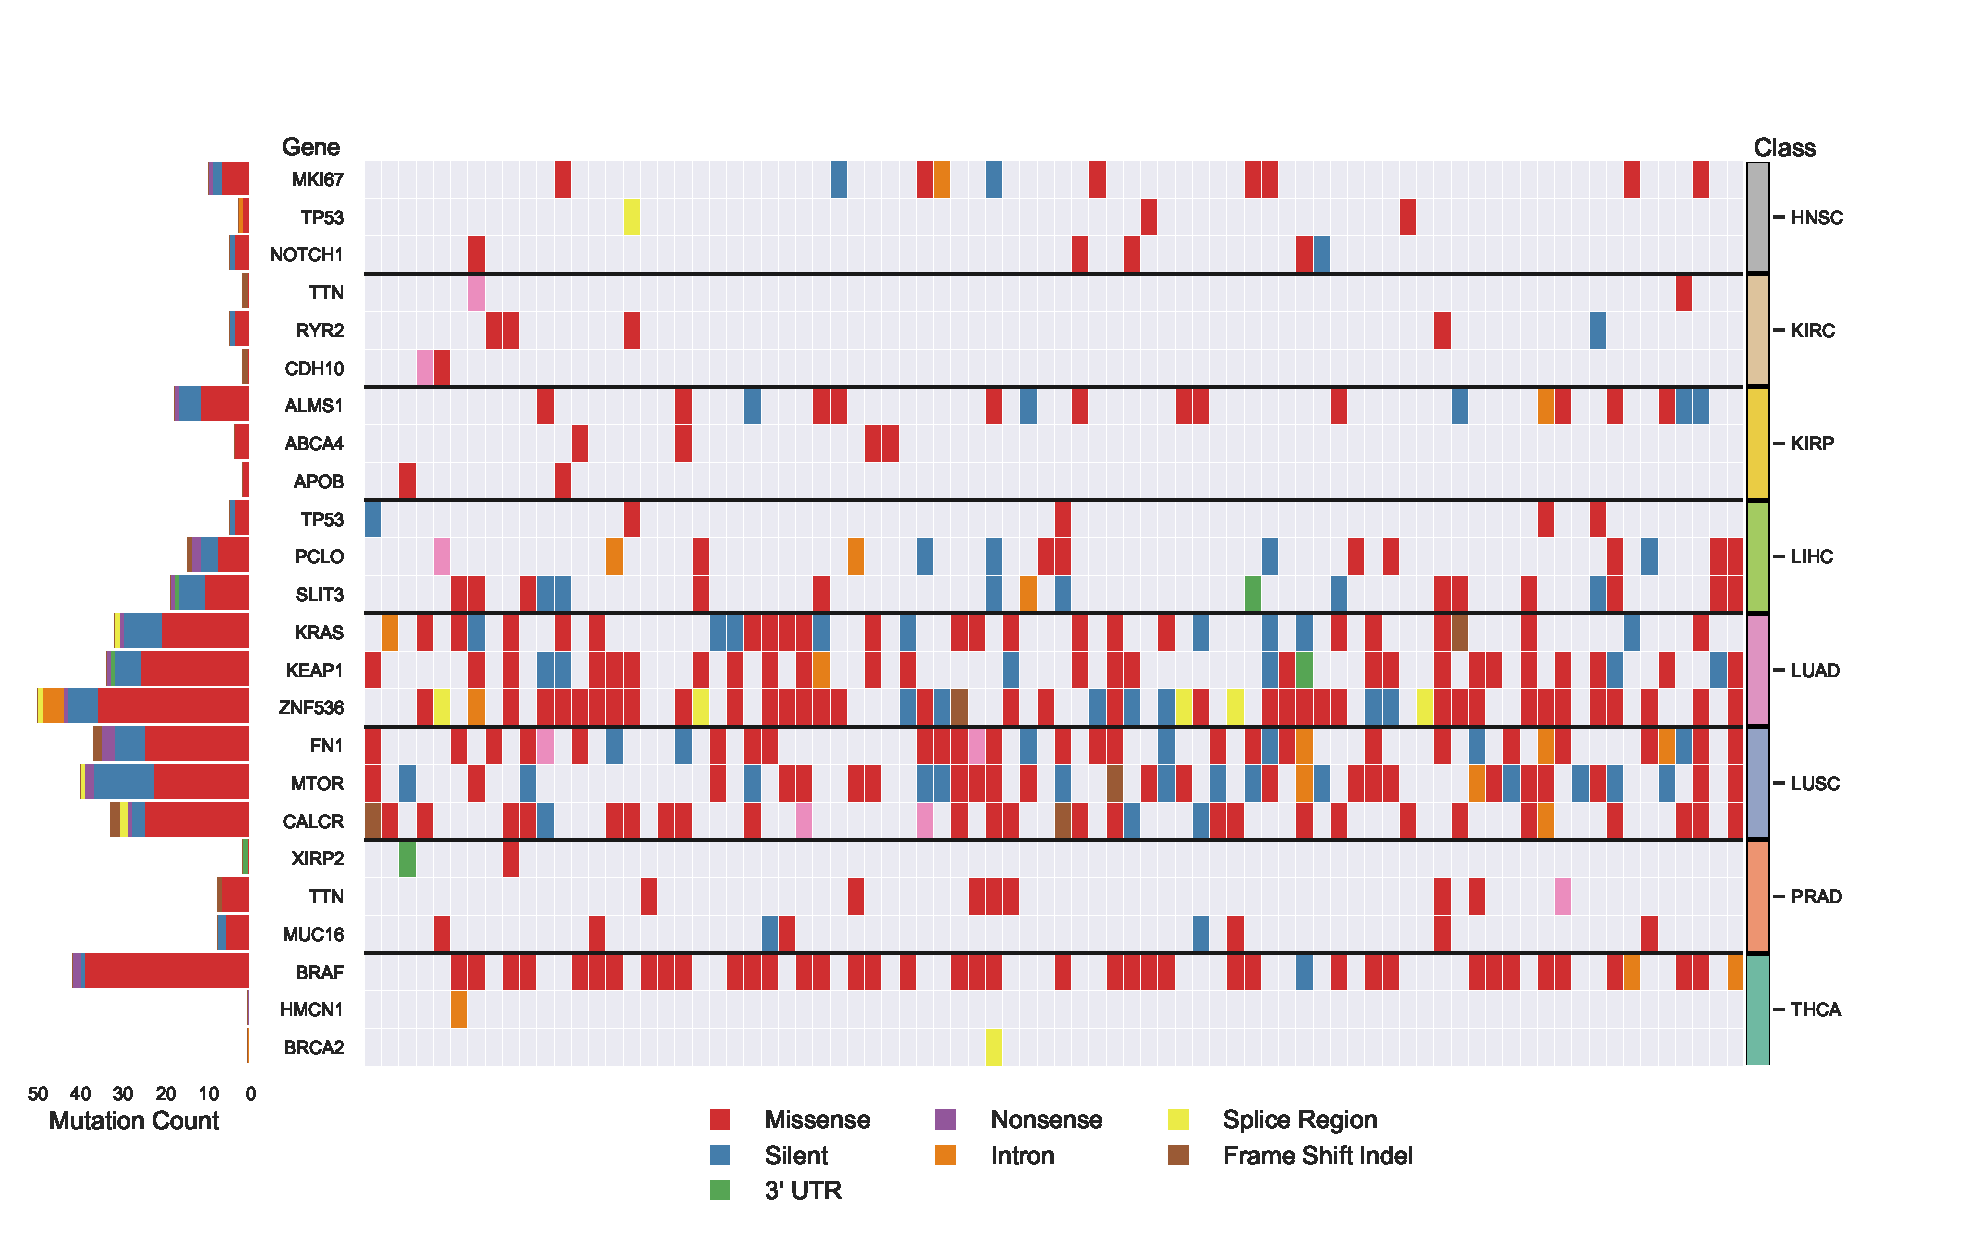
\includegraphics[width=\textwidth]{img/oncoplot.eps}
    \caption{Top 3 explanatory single nucleotide variations for each cancer class.}
    \label{fig:oncoplot}
\end{figure}

%%Fix plot, pink color not in the legend

The genetic variations of the top 3 explanatory SNV gene regions were visualized across the cell samples for each cancer class on Fig. \ref{fig:oncoplot}. Each column represents a sample and each row a different gene. The fields are labeled to indicate the category of SNV that is present in the region of the respective gene. The left barplot shows the frequency of variations for each gene, and the associated cancer class is labeled on the right. The mutation frequency of the top 3 SNV gene regions varied widely across the cancer types. The lung cancers LUAD and LUSC had the highest presence of SNVs and the remaining cancers had very sparse variations across cell samples. An exception to this appeared for the BRAF gene in the THCA cancer cell samples. The genetic aberrations of all top three genes have been implicated in the development of various cancers, but genetic variations in HMCN1 and BRCA2 were only found in one case each. \cite{mersch2015cancers,kikutake2018intratumor,kebebew2007prevalence}. Genetic variations in BRAF were found in more than half of the cell samples, the majority of which were missense mutations. BRAF is a protein coding gene involved in the regulation of signalling pathways that influence cell division, differentiation, and secretion. Mutations in this gene are recurrent in THCA and the missense point mutation in which a single nucleotide change results in valine 600 to glutamic acid (V600E) is the most prevalent \cite{xing2013association}. Although THCA has a low mortality rate, the presence of the V600E mutation is associated with faster cancer growth and a higher death rate \cite{xing2013association}. Accordingly, the interpretable local explanations derived from LIME indicate that the dGMU model draws from clinically relevant information. This trend is found across the different cancer types. The LIME algorithm indicated SNVs in cancer related genes in all cancer types which provides reasonable explanations that a domain expert can use to understand the prediction of the dGMU model. 
